\chapter{AVALIAÇÃO E RESULTADOS}
\label{cap:resultados}

Este capítulo apresenta e discute os resultados obtidos segundo o protocolo da Seção \ref{sec:protocolo}. A Seção \ref{sec:res-robustez} analisa a robustez técnica ao longo das iterações, a Seção \ref{sec:res-desempenho} trata do desempenho computacional, a Seção \ref{sec:res-corpus} apresenta os resultados da validação dos 29 planos, a Seção \ref{sec:res-oraculo} mede a concordância com o oráculo estrutural e a Seção \ref{sec:res-erros} analisa os erros do sistema. A Seção \ref{sec:res-semestres} amplia a avaliação para os 120 planos de quatro semestres, de 2024/1 a 2025/2, e a Seção \ref{sec:res-discussao} discute os resultados em conjunto. Salvo indicação contrária, os números das Seções \ref{sec:res-robustez} a \ref{sec:res-erros} referem-se à execução da versão final sobre os planos de 2024/1, realizada em 19 de outubro de 2026.

\section{Robustez técnica ao longo das iterações}
\label{sec:res-robustez}

A primeira dimensão avaliada é a robustez técnica, pois um sistema que falha ao processar os planos não pode ter seus resultados avaliados nas demais dimensões. A Figura \ref{fig:evolucao} mostra a proporção de planos que receberam o status ERRO em cada data de execução registrada na planilha de resultados. Nas datas com mais de uma execução, como 25/08, o valor agrega todas as execuções do dia.

\begin{figure}[htbp]
\centering
\caption{Proporção de planos com status ERRO por data de execução}
\label{fig:evolucao}
% Dados: aba Validações da planilha (registros por data de execução) e execução de 19/10/2026
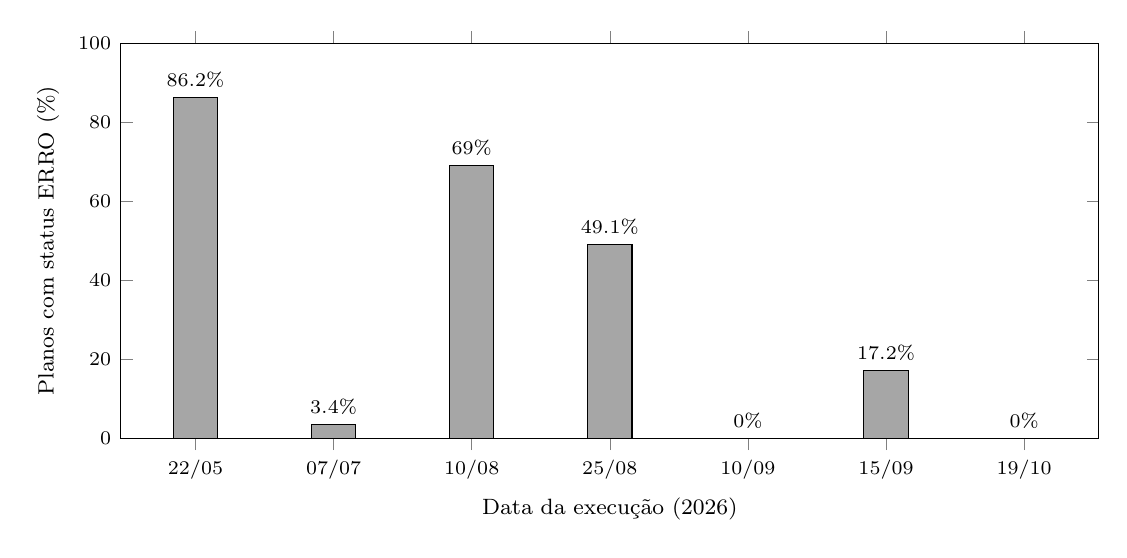
\begin{tikzpicture}
\begin{axis}[
  ybar,
  width=14cm, height=6.6cm,
  bar width=16pt,
  ymin=0, ymax=100,
  ylabel={Planos com status ERRO (\%)},
  symbolic x coords={22/05,07/07,10/08,25/08,10/09,15/09,19/10},
  xtick=data,
  xlabel={Data da execução (2026)},
  nodes near coords={\pgfmathprintnumber[fixed,precision=1]{\pgfplotspointmeta}\%},
  nodes near coords style={font=\scriptsize},
  ticklabel style={font=\scriptsize},
  label style={font=\footnotesize},
  enlarge x limits=0.09,
]
\addplot[fill=black!35, draw=black] coordinates {
  (22/05,86.2) (07/07,3.4) (10/08,69.0) (25/08,49.1) (10/09,0) (15/09,17.2) (19/10,0)};
\end{axis}
\end{tikzpicture}

\legend{Fonte: Elaborado pelo autor (2026), a partir da planilha de resultados (348 registros) e da execução de 19/10/2026.}
\end{figure}

A análise das mensagens de erro registradas permitiu identificar quatro causas de falha, resumidas na Tabela \ref{tab:falhas} com as correções correspondentes.

\begin{table}[H]
\centering
\caption{Causas de falha identificadas e correções aplicadas}
\label{tab:falhas}
\footnotesize
\begin{tabular}{@{}L{3.4cm}L{4.7cm}L{6.3cm}@{}}
\toprule
\rowcolor[HTML]{EFEFEF}
\textbf{Sintoma} & \textbf{Causa} & \textbf{Correção} \\ \midrule
Resposta vazia ou JSON truncado (``\textit{Unexpected end of JSON input}'') & Requisições simultâneas sobrecarregavam o servidor de inferência, que interrompia respostas & Processamento em blocos, uma requisição por vez, com até três tentativas \\
JSON malformado (``\textit{Expected ',' or '\}'}'') & O modelo produzia texto fora da sintaxe JSON & Saída estruturada com esquema JSON no parâmetro \texttt{format} \\
Respostas em outro idioma ou com JSON sem relação com o pedido & O \textit{prompt} (cerca de 5.100 \textit{tokens} à época) excedia o contexto padrão de 4.096 \textit{tokens} e era truncado & Definição explícita do contexto (12.288 e, depois, 8.192 \textit{tokens}) e redução do \textit{prompt} \\
Estouro do tempo limite (\textit{timeout}) & Geração lenta, com parte do modelo fora da GPU e queda de desempenho do equipamento & Contexto de 8.192, \textit{FlashAttention} e \textit{KV cache} em 8 bits \\ \bottomrule
\end{tabular}
\legend{Fonte: Elaborado pelo autor (2026).}
\end{table}

A causa mais frequente foi a resposta vazia ou truncada, responsável por todas as falhas de 22/05 e de 10/08 e por 55 das 57 falhas de 25/08. O problema não estava no modelo, mas na forma de chamá-lo: o n8n enviava as requisições de todos os planos quase ao mesmo tempo, e o servidor as enfileirava e interrompia. A solução foi controlar a concorrência no próprio fluxo, com o laço de blocos da Figura \ref{fig:pipeline}. O comportamento intermitente, com poucas falhas em 07/07 e muitas novamente em 10/08, é compatível com uma falha dependente da carga sobre o servidor, e não de planos específicos. As duas falhas de 07/07 foram de outro tipo, JSON malformado, eliminado com a adoção da saída estruturada.

O truncamento do contexto foi o problema mais difícil de diagnosticar, pois não gerava erro: o Ollama descartava silenciosamente a parte do \textit{prompt} que excedia o contexto padrão, e o modelo, sem parte das instruções, respondia em outro idioma ou produzia um JSON sem relação com o pedido. O episódio ilustra uma característica dos sistemas com LLMs: falhas de configuração podem se manifestar como respostas plausíveis e incorretas, e não como erros explícitos, o que reforça a importância do registro detalhado das execuções defendido pelas práticas de MLOps \cite{Kreuzberger2023}.

Na execução de 15/09, cinco planos falharam por estouro do tempo limite, então de 600 segundos. Os metadados do Ollama mostram que a velocidade de geração caiu de 18,1 para 5,6 \textit{tokens} por segundo em relação à execução de 10/09, com a mesma configuração de inferência, o que indica uma queda de desempenho do equipamento, como o estrangulamento térmico ou a entrada em modo de economia de energia, e não um problema do fluxo. A otimização de memória da iteração de outubro, discutida na próxima seção, e o tempo limite menor, de 180 segundos, com retentativas, tornaram o sistema menos sensível a essas variações. Na execução final, nenhum dos 29 planos falhou.

\section{Desempenho computacional}
\label{sec:res-desempenho}

Eliminadas as falhas técnicas, a questão seguinte é se o sistema processa o lote em tempo compatível com o uso real. A Tabela \ref{tab:desempenho} resume os metadados de inferência da execução final. Cada plano gerou, em média, um \textit{prompt} de 3.248 \textit{tokens} e uma resposta de 274 \textit{tokens}. A leitura do \textit{prompt} levou em média 1,6 segundo e a geração da resposta, 9,9 segundos, totalizando 11,5 segundos de inferência por plano. A velocidade média de geração foi de 27,6 \textit{tokens} por segundo. O lote completo de 29 planos, incluindo a listagem e o \textit{download} dos arquivos, a extração, as chamadas ao modelo e a gravação na planilha, foi processado em 8 minutos e 54 segundos, abaixo do limite de 30 minutos estabelecido no RNF03. Essa execução usou a versão com Google Drive e Google Sheets; na versão final, com pastas locais, a leitura dos arquivos e a gravação dos resultados deixam de passar pela rede, e o tempo total continua dominado pela inferência, que respondeu por cerca de 5,6 dos 8,9 minutos.

\begin{table}[H]
\centering
\caption{Estatísticas de inferência por plano na execução final (n = 29)}
\label{tab:desempenho}
\footnotesize
\begin{tabular}{@{}lrrrrr@{}}
\toprule
\rowcolor[HTML]{EFEFEF}
\textbf{Medida} & \textbf{Mínimo} & \textbf{Máximo} & \textbf{Média} & \textbf{Mediana} & \textbf{Desvio-padrão} \\ \midrule
Páginas do PDF & 3 & 5 & 3,4 & 3 & 0,6 \\
Caracteres extraídos & 4.520 & 11.436 & 7.048 & 6.770 & 1.700 \\
\textit{Tokens} do \textit{prompt} & 2.481 & 4.522 & 3.248 & 3.120 & 558 \\
\textit{Tokens} da resposta & 250 & 347 & 274 & 269 & 18 \\
Tempo de leitura do \textit{prompt} (s) & 0,8 & 11,3 & 1,6 & 1,2 & 1,9 \\
Tempo de geração (s) & 8,9 & 12,3 & 9,9 & 9,8 & 0,6 \\ \bottomrule
\end{tabular}
\legend{Fonte: Elaborado pelo autor (2026), a partir dos metadados do Ollama.}
\end{table}

O tamanho da resposta variou pouco, pois o esquema JSON fixa sua estrutura, e o tempo de geração acompanhou essa estabilidade, com desvio-padrão de apenas 0,6 segundo. O tempo de leitura do \textit{prompt} teve um valor atípico de 11,3 segundos em um dos planos; nos demais, ficou entre 0,8 e 1,9 segundo.

A Figura \ref{fig:desempenho} compara a velocidade de geração em três execuções sobre o mesmo corpus. Entre 10/09 e 19/10, a velocidade passou de 18,1 para 27,6 \textit{tokens} por segundo, um ganho de 52\%, e o tempo total do lote caiu de 46 minutos para menos de 9 minutos. O ganho decorre da combinação de três mudanças na iteração de outubro: a redução do contexto de 12.288 para 8.192 \textit{tokens}, viabilizada pela segmentação mais precisa, que eliminou trechos desnecessários do \textit{prompt}; o \textit{FlashAttention}; e a quantização do \textit{KV cache} em 8 bits. Juntas, essas mudanças reduziram a memória ocupada pelo contexto; na configuração final, o Ollama reportou 92\% do modelo alocado na GPU de 6 GB, com o restante na CPU. A execução de 15/09 é mostrada como referência do efeito da degradação do equipamento discutida na seção anterior.

\begin{figure}[htbp]
\centering
\caption{Velocidade de geração por configuração}
\label{fig:desempenho}
% Dados: metadados das respostas do Ollama nas execuções de 10/09, 15/09 e 19/10/2026 (29 planos cada)
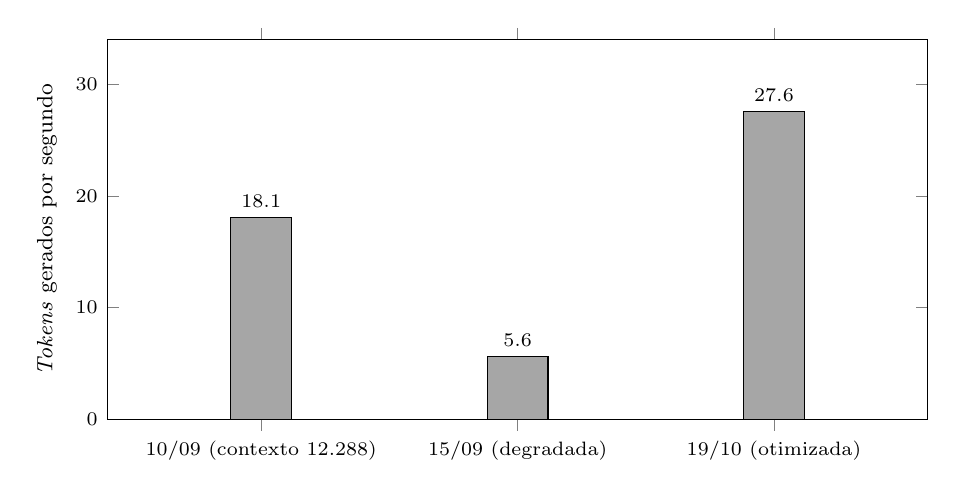
\begin{tikzpicture}
\begin{axis}[
  ybar,
  width=12cm, height=6.4cm,
  bar width=22pt,
  ymin=0, ymax=34,
  ylabel={\textit{Tokens} gerados por segundo},
  symbolic x coords={10/09,15/09,19/10},
  xtick=data,
  xticklabels={{10/09 (contexto 12.288)},{15/09 (degradada)},{19/10 (otimizada)}},
  nodes near coords={\pgfmathprintnumber[fixed,precision=1]{\pgfplotspointmeta}},
  nodes near coords style={font=\scriptsize},
  ticklabel style={font=\scriptsize},
  label style={font=\footnotesize},
  enlarge x limits=0.3,
]
\addplot[fill=black!35, draw=black] coordinates {(10/09,18.1) (15/09,5.6) (19/10,27.6)};
\end{axis}
\end{tikzpicture}

\legend{Fonte: Elaborado pelo autor (2026), a partir dos metadados do Ollama.}
\end{figure}

Extrapolando a média de 11,5 segundos de inferência por plano, a validação dos planos de todos os cursos de um campus, na casa das centenas por semestre, levaria menos de uma hora no mesmo equipamento, executada de madrugada pelo agendamento diário. O desempenho obtido é, portanto, compatível com o uso real, sem custo por requisição e sem envio dos documentos a serviços externos.

\section{Resultados da validação do corpus}
\label{sec:res-corpus}

Com o sistema estável e com desempenho adequado, esta seção apresenta o que ele apontou sobre os planos. Na execução final, 11 planos (37,9\%) foram considerados conformes (OK), 3 (10,3\%) pendentes e 15 (51,7\%) reprovados. A Figura \ref{fig:criterios} detalha o resultado por critério.

\begin{figure}[htbp]
\centering
\caption{Resultado por critério na execução final (29 planos)}
\label{fig:criterios}
% Dados: dados/validacoes_2026-10-19.csv (execução de 19/10/2026, 29 planos)
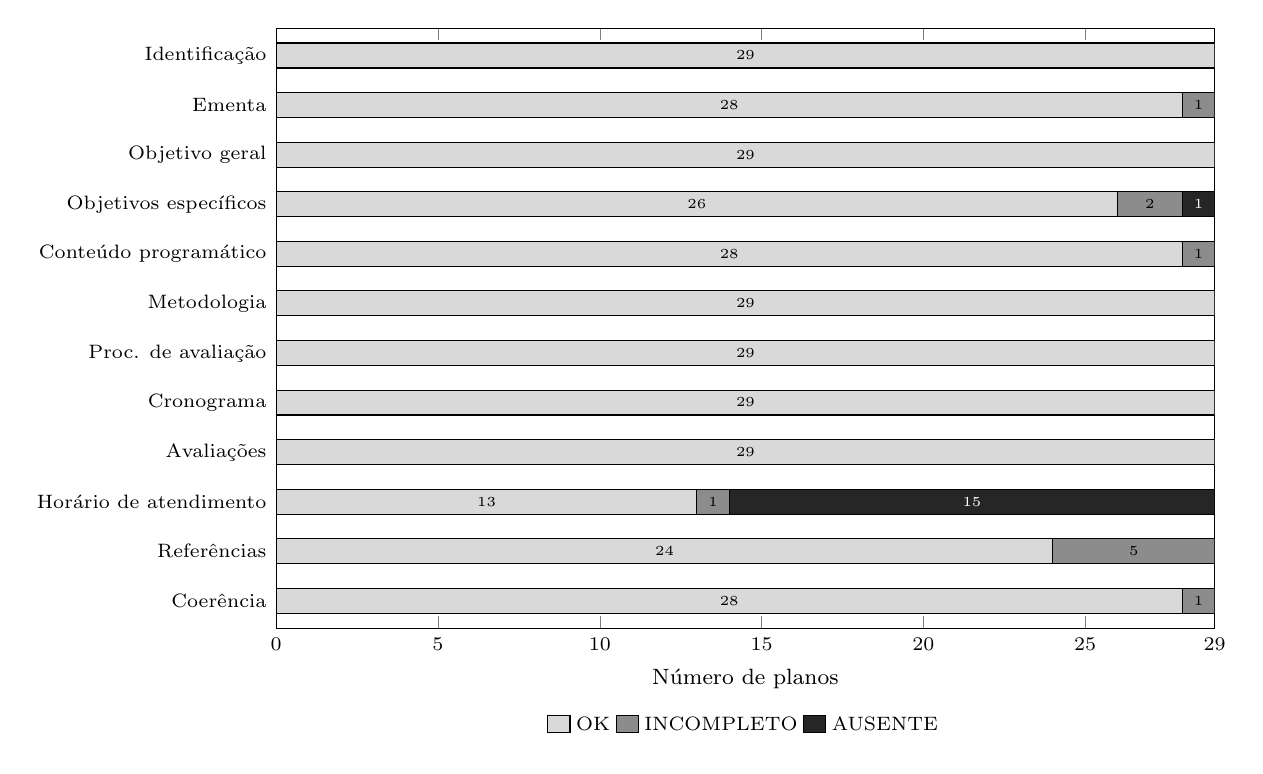
\begin{tikzpicture}
\begin{axis}[
  xbar stacked,
  width=13.5cm, height=9.2cm,
  bar width=9pt,
  xmin=0, xmax=29,
  xtick={0,5,10,15,20,25,29},
  xlabel={Número de planos},
  ytick=data,
  yticklabels={Identificação,Ementa,Objetivo geral,Objetivos específicos,Conteúdo programático,Metodologia,Proc. de avaliação,Cronograma,Avaliações,Horário de atendimento,Referências,Coerência},
  y dir=reverse,
  ticklabel style={font=\scriptsize},
  label style={font=\footnotesize},
  legend style={at={(0.5,-0.13)}, anchor=north, legend columns=3, font=\scriptsize, draw=none},
  nodes near coords={\pgfmathprintnumber{\pgfplotspointmeta}},
  nodes near coords style={font=\tiny},
  point meta=explicit symbolic,
  enlarge y limits=0.05,
]
\addplot[fill=black!15, draw=black] coordinates {
  (29,1) [29] (28,2) [28] (29,3) [29] (26,4) [26] (28,5) [28] (29,6) [29]
  (29,7) [29] (29,8) [29] (29,9) [29] (13,10) [13] (24,11) [24] (28,12) [28]};
\addplot[fill=black!45, draw=black] coordinates {
  (0,1) [] (1,2) [1] (0,3) [] (2,4) [2] (1,5) [1] (0,6) []
  (0,7) [] (0,8) [] (0,9) [] (1,10) [1] (5,11) [5] (1,12) [1]};
\addplot[fill=black!85, draw=black, nodes near coords style={font=\tiny, text=white}] coordinates {
  (0,1) [] (0,2) [] (0,3) [] (1,4) [1] (0,5) [] (0,6) []
  (0,7) [] (0,8) [] (0,9) [] (15,10) [15] (0,11) [] (0,12) []};
\legend{OK, INCOMPLETO, AUSENTE}
\end{axis}
\end{tikzpicture}

\legend{Fonte: Elaborado pelo autor (2026).}
\end{figure}

Seis critérios foram considerados conformes em todos os planos: identificação, objetivo geral, metodologia, procedimentos de avaliação, cronograma e avaliações. O resultado é esperado para identificação e cronograma, cuja estrutura é gerada pelo próprio SIGAA, e indica que os docentes descrevem de forma consistente a metodologia e os instrumentos de avaliação.

O critério com mais não conformidades foi o horário de atendimento, ausente em 15 planos e incompleto em um. Todos os 15 planos reprovados têm o horário de atendimento ausente, e em 9 deles essa é a única não conformidade. O dado é relevante para a gestão do curso: trata-se de uma informação de interesse direto dos estudantes, de preenchimento simples, cuja ausência em mais da metade dos planos dificilmente seria percebida sem uma verificação sistemática.

O segundo critério mais apontado foi o de referências, incompleto em 5 planos. Em quatro deles faltavam referências complementares: três planos tinham 4 e um não tinha nenhuma das 5 exigidas. No quinto, a proporção estava invertida, com 5 referências básicas e apenas 3 complementares. Os demais apontamentos foram pontuais: objetivos específicos em três planos, e ementa, conteúdo programático e coerência em um plano cada.

\section{Concordância com o oráculo estrutural}
\label{sec:res-oraculo}

Os resultados da seção anterior só são úteis se os apontamentos estiverem corretos. O critério de horário de atendimento, o mais apontado, é também o único que pode ser conferido por uma referência independente do modelo. Para esse critério, o oráculo estrutural descrito na Seção \ref{sec:protocolo} identificou 15 planos com o campo vazio e 14 com conteúdo. A Tabela \ref{tab:confusao} apresenta a matriz de confusão do sistema em relação a esse oráculo, considerando como positivo o plano não conforme, isto é, com status INCOMPLETO ou AUSENTE.

\begin{table}[H]
\centering
\caption{Matriz de confusão do critério horário de atendimento}
\label{tab:confusao}
\footnotesize
\begin{tabular}{@{}lccc@{}}
\toprule
\rowcolor[HTML]{EFEFEF}
 & \textbf{Sistema: não conforme} & \textbf{Sistema: conforme} & \textbf{Total} \\ \midrule
\textbf{Oráculo: campo vazio} & 15 (VP) & 0 (FN) & 15 \\
\textbf{Oráculo: campo preenchido} & 1 (FP) & 13 (VN) & 14 \\
\textbf{Total} & 16 & 13 & 29 \\ \bottomrule
\end{tabular}
\legend{Fonte: Elaborado pelo autor (2026).}
\end{table}

O sistema detectou todos os 15 campos vazios, o que corresponde a um \textit{recall} de 100\%, e apontou um único plano cujo campo estava preenchido, resultando em precisão de 93,8\%, $F_1$ de 0,968 e acurácia de 96,6\%. O Kappa de Cohen foi de 0,931, o que corresponde a concordância quase perfeita na escala de \citeonline{Landis1977}.

O único falso positivo em relação ao oráculo, o plano P19, merece atenção. Seu campo contém a frase ``conforme horário disponibilizado publicamente'', que não informa dia nem horário. Pela regra do critério (Tabela \ref{tab:criterios}), o plano é de fato não conforme, de modo que o apontamento está correto quanto à conformidade, e a divergência decorre da limitação do oráculo, que apenas verifica se o campo está vazio. O erro do modelo está na categoria: deveria ter atribuído INCOMPLETO, pois há conteúdo relacionado, mas atribuiu AUSENTE, contrariando a instrução explícita do \textit{prompt}. Considerando a regra do critério, e não apenas o oráculo estrutural, o sistema acertou a conformidade dos 29 planos e errou a categoria em dois: o P19, como descrito, e o P21, que tem o campo vazio e recebeu INCOMPLETO em vez de AUSENTE.

\section{Análise de erros}
\label{sec:res-erros}

Para os demais critérios, que não têm oráculo estrutural, a correção dos apontamentos foi verificada manualmente. Todos os apontamentos da execução final, além dos de horário de atendimento, foram confrontados com o texto extraído dos PDFs. A Tabela \ref{tab:erros} apresenta o resultado dessa verificação.

\begin{table}[H]
\centering
\caption{Verificação dos apontamentos da execução final (exceto horário de atendimento)}
\label{tab:erros}
\footnotesize
\begin{tabular}{@{}L{1.1cm}L{2.8cm}L{2.4cm}L{4.3cm}L{3.6cm}@{}}
\toprule
\rowcolor[HTML]{EFEFEF}
\textbf{Plano} & \textbf{Critério} & \textbf{Sistema} & \textbf{Conteúdo no PDF} & \textbf{Avaliação} \\ \midrule
P05 & Objetivos específicos & AUSENTE & ``Objetivos: Não Cadastrado!'' & Correto \\
P05 & Conteúdo programático & INCOMPLETO & ``Não Cadastrado!'' & Não conformidade correta; categoria deveria ser AUSENTE \\
P05 & Coerência & INCOMPLETO & Sem objetivos para comparar & Correto \\
P05 & Objetivo geral & OK & ``Não Cadastrado!'' & Falso negativo \\
P20, P21 & Objetivos específicos & INCOMPLETO & Objetivo em parágrafo único, sem objetivos específicos & Não conformidade correta \\
P27 & Ementa & INCOMPLETO & ``A cadastrar'' & Não conformidade correta; categoria deveria ser AUSENTE \\
P11, P23, P25, P28, P29 & Referências & INCOMPLETO & Contagens conferidas no texto & Correto \\ \bottomrule
\end{tabular}
\legend{Fonte: Elaborado pelo autor (2026).}
\end{table}

Todos os 11 apontamentos verificados correspondem a não conformidades reais. Em dois deles, porém, a categoria atribuída foi INCOMPLETO quando o campo continha apenas um texto provisório do SIGAA, situação que deveria ser classificada como AUSENTE. Esse padrão, somado aos dois erros de categoria do horário de atendimento, mostra que o modelo distingue bem a presença de um problema, mas é menos confiável na escolha entre INCOMPLETO e AUSENTE. O caso dos planos P20 e P21, duas turmas do mesmo componente com o campo de horário igualmente vazio, que receberam AUSENTE e INCOMPLETO respectivamente, mostra que essa escolha pode variar mesmo com temperatura 0,1, quando outras partes do \textit{prompt}, como o cronograma, diferem. Como a categoria determina se o plano é REPROVADO ou PENDENTE, essa instabilidade afeta o status geral: o P21 foi classificado como PENDENTE, enquanto o P20, praticamente idêntico, foi REPROVADO.

Foi identificado um falso negativo: o objetivo geral do plano P05 foi considerado OK, embora contivesse apenas o texto provisório ``Não Cadastrado!''. O erro não é do modelo, mas da regra determinística RN04, que considera conforme qualquer texto preenchido. Uma busca por textos provisórios em todo o corpus confirmou que esse foi o único caso em que um texto provisório foi aceito como conteúdo válido; nos outros dois (conteúdo programático do P05 e ementa do P27), o modelo apontou corretamente a não conformidade.

Por fim, a análise revelou um problema de consistência na observação geral, o resumo em uma frase produzido pelo modelo. Em 18 dos 24 planos cujo critério de referências foi considerado conforme, a observação geral mencionava algum problema com as referências, como ``faltam referências básicas''. A contradição ocorre porque a observação geral é escrita pelo modelo antes da aplicação das regras determinísticas, e o modelo, mesmo recebendo a contagem verificada, tende a comentar as referências de forma equivocada. Embora não altere nenhum status, a contradição aparece no \textit{dashboard} e pode confundir o avaliador. A correção indicada é gerar a observação geral por código, a partir dos status finais dos critérios.

\section{Ampliação para quatro semestres}
\label{sec:res-semestres}

As seções anteriores avaliaram o sistema em profundidade sobre os planos de 2024/1. Para verificar se o comportamento se mantém em outros semestres e observar a evolução da conformidade dos planos ao longo do tempo, a versão final, já com armazenamento local, foi executada em 4 de novembro de 2026 sobre os planos dos semestres 2024/1, 2024/2, 2025/1 e 2025/2, disponibilizados pelo orientador em uma pasta compartilhada. A pasta continha 126 arquivos. Seis deles, de 2024/2 a 2025/2, são documentos digitalizados, sem camada de texto, e não puderam ser processados, pois o sistema não realiza reconhecimento óptico de caracteres. Os 120 restantes seguem o modelo do SIGAA e foram todos processados. Os planos foram identificados por códigos de S1-P01 a S4-P28, em que S1 a S4 indicam o semestre, e os resultados anonimizados estão no arquivo \texttt{dados/validacoes\_2026-11-04.csv} do repositório.

\subsection{Resultados por semestre}

A Figura \ref{fig:semestres} apresenta o status geral dos planos em cada semestre. No conjunto, 36 planos (30,0\%) foram considerados conformes, 21 (17,5\%) pendentes e 63 (52,5\%) reprovados. A proporção de planos reprovados variou entre 41,2\%, em 2024/2, e 65,5\%, em 2025/1.

\begin{figure}[htbp]
\centering
\caption{Status geral dos planos por semestre}
\label{fig:semestres}
% Dados: dados/validacoes_2026-11-04.csv (execução de 04/11/2026, 120 planos)
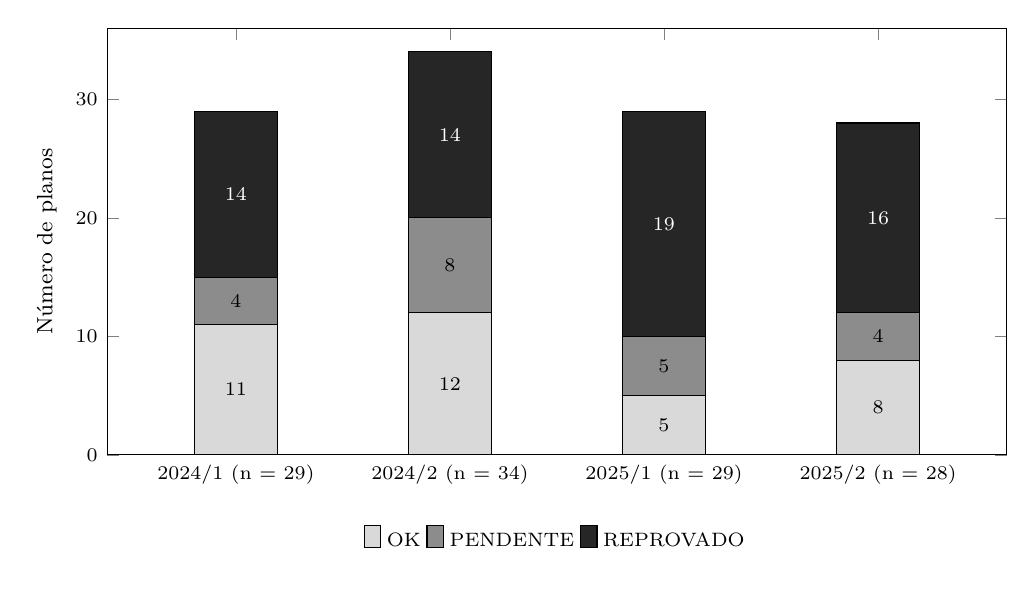
\begin{tikzpicture}
\begin{axis}[
  ybar stacked,
  width=13cm, height=7cm,
  bar width=30pt,
  ymin=0, ymax=36,
  ylabel={Número de planos},
  symbolic x coords={2024/1,2024/2,2025/1,2025/2},
  xtick=data,
  xticklabels={{2024/1 (n = 29)},{2024/2 (n = 34)},{2025/1 (n = 29)},{2025/2 (n = 28)}},
  nodes near coords={\pgfmathprintnumber{\pgfplotspointmeta}},
  nodes near coords style={font=\scriptsize},
  ticklabel style={font=\scriptsize},
  label style={font=\footnotesize},
  legend style={at={(0.5,-0.15)}, anchor=north, legend columns=3, font=\scriptsize, draw=none},
  enlarge x limits=0.2,
]
\addplot[fill=black!15, draw=black] coordinates {(2024/1,11) (2024/2,12) (2025/1,5) (2025/2,8)};
\addplot[fill=black!45, draw=black] coordinates {(2024/1,4) (2024/2,8) (2025/1,5) (2025/2,4)};
\addplot[fill=black!85, draw=black, nodes near coords style={font=\scriptsize, text=white}] coordinates {(2024/1,14) (2024/2,14) (2025/1,19) (2025/2,16)};
\legend{OK, PENDENTE, REPROVADO}
\end{axis}
\end{tikzpicture}

\legend{Fonte: Elaborado pelo autor (2026), a partir da execução de 04/11/2026.}
\end{figure}

O padrão observado em 2024/1 se repete nos demais semestres: o horário de atendimento é, de longe, o critério com mais apontamentos, não conforme em 69 dos 120 planos (57,5\%), seguido pelas referências, incompletas em 17 planos, e pelos objetivos específicos, com 16 apontamentos. Em 43 planos, o horário de atendimento é a única não conformidade. Identificação e objetivo geral foram considerados conformes em todos os planos, e metodologia, cronograma e coerência tiveram no máximo três apontamentos cada.

\subsection{Horário de atendimento e referência a páginas externas}

A ampliação revelou uma mudança na forma de preencher o horário de atendimento. Em 2024/1, os planos não conformes tinham, com uma exceção, o campo vazio. A partir de 2024/2, muitos docentes passaram a preenchê-lo apenas com uma referência externa, em geral o endereço da página em que o campus publica os planos de trabalho docente (\texttt{videira.ifc.edu.br/ptd-e-rtd}), sem indicar dia nem horário. A Tabela \ref{tab:horario-semestres} resume essa mudança.

\begin{table}[H]
\centering
\caption{Conteúdo do campo de horário de atendimento nos planos não conformes}
\label{tab:horario-semestres}
\footnotesize
\begin{tabular}{@{}lccccc@{}}
\toprule
\rowcolor[HTML]{EFEFEF}
\textbf{Conteúdo do campo} & \textbf{2024/1} & \textbf{2024/2} & \textbf{2025/1} & \textbf{2025/2} & \textbf{Total} \\ \midrule
Vazio & 15 & 8 & 5 & 7 & 35 \\
Endereço da página de PTD & 0 & 6 & 13 & 10 & 29 \\
Outra referência externa (``conforme horário divulgado'') & 1 & 1 & 3 & 0 & 5 \\ \midrule
\textbf{Total de planos não conformes} & \textbf{16} & \textbf{15} & \textbf{21} & \textbf{17} & \textbf{69} \\ \bottomrule
\end{tabular}
\legend{Fonte: Elaborado pelo autor (2026).}
\end{table}

Essa mudança tem dois efeitos sobre a avaliação. O primeiro é sobre o oráculo estrutural da Seção \ref{sec:res-oraculo}, que considera conforme qualquer campo preenchido. Sobre os 120 planos, o sistema manteve \textit{recall} de 100\%, mas a precisão em relação a esse oráculo caiu para 50,7\% e o Kappa de Cohen para 0,47, porque os 34 campos com referência externa contam como falsos positivos. Conferidos um a um, porém, nenhum desses 34 campos informa dia ou horário, de modo que todos são não conformes pela regra do critério (Tabela \ref{tab:criterios}), e todos os 51 planos considerados conformes informam dia ou horário explicitamente. Pela regra, o sistema acertou a conformidade do horário de atendimento nos 120 planos. Repete-se, contudo, o erro de categoria já observado no P19: em 33 dos 34 campos com referência externa, o modelo atribuiu AUSENTE, quando deveria atribuir INCOMPLETO. O episódio mostra que um oráculo estrutural válido em um semestre pode deixar de sê-lo quando a prática de preenchimento muda, e reforça a necessidade da anotação humana prevista no protocolo.

O segundo efeito é normativo. A Organização Didática exige que o plano informe o horário de atendimento \cite{ifc2022}, mas não diz se uma referência à página de PTD do campus atende a essa exigência. A decisão cabe à coordenação e ao NDE, e o impacto é grande: se a referência externa fosse aceita, o número de planos reprovados nos quatro semestres cairia de 63 para 30, e o de planos conformes subiria de 36 para 63. A regra do critério pode ser ajustada no \textit{prompt} em qualquer dos dois sentidos, mas a escolha é institucional, e não técnica.

\subsection{Reprodutibilidade e desempenho}

Os 29 planos de 2024/1 foram processados novamente nessa execução, com a mesma configuração de inferência, o que permitiu medir a reprodutibilidade dos resultados. Das 377 classificações (12 critérios e o status geral de cada plano), 374 (99,2\%) foram idênticas às da execução de 19 de outubro. As três diferenças envolvem, mais uma vez, a escolha entre INCOMPLETO e AUSENTE e mudaram o status geral de um plano, o P20, de REPROVADO para PENDENTE.

O desempenho, por outro lado, foi bem inferior ao da Seção \ref{sec:res-desempenho}. Com outros programas abertos ocupando parte da memória da GPU, o Ollama alocou 14\% do modelo na CPU, contra 8\% na execução de outubro, e cada plano passou a levar de 30 a 60 segundos de inferência. Essa lentidão expôs uma fragilidade do fluxo: o nó de requisição envia um plano por segundo dentro de cada bloco de 10, sem aguardar a resposta anterior, e o servidor de inferência os enfileira. Com 11,5 segundos por plano, o último do bloco termina antes do tempo limite de 180 segundos; com 30 segundos ou mais, não termina. Na primeira tentativa, 55 planos receberam o status ERRO por estouro do tempo limite. Esses planos foram reprocessados com o tempo limite ampliado para 900 segundos, e todos foram avaliados. O episódio mostra que o controle de concorrência descrito na Tabela \ref{tab:falhas} depende do desempenho do equipamento, e que o fluxo deveria aguardar cada resposta antes de enviar o plano seguinte, o que é indicado como trabalho futuro.

\section{Discussão}
\label{sec:res-discussao}

As seções anteriores analisaram cada dimensão da avaliação separadamente. Considerados em conjunto, os resultados permitem responder ao problema de pesquisa sob três aspectos. Quanto à viabilidade técnica, o sistema processou o corpus completo sem falhas, em menos de 9 minutos, em um computador portátil com GPU de 6 GB e sem custos por requisição. A evolução das iterações mostra, porém, que essa robustez não veio do modelo, mas da engenharia em torno dele: controle de concorrência, saída estruturada, dimensionamento do contexto e registro detalhado das execuções. Esse resultado é coerente com a visão de \citeonline{Kreuzberger2023} de que sistemas com componentes de aprendizado de máquina dependem tanto da infraestrutura e da operação quanto do modelo.

Quanto à qualidade da triagem, o sistema não deixou de apontar nenhuma das não conformidades verificáveis por oráculo e todos os seus apontamentos verificados correspondiam a problemas reais, com um único falso negativo identificado, causado por uma regra determinística e não pelo modelo. A principal fragilidade está na distinção entre INCOMPLETO e AUSENTE. Para uma ferramenta de triagem, cujo objetivo é dirigir a atenção do avaliador, a detecção do problema é mais importante que sua categoria, mas a categoria afeta o status geral e, portanto, a priorização dos planos. Esses resultados estão alinhados com a literatura sobre LLMs como avaliadores, que relata boa concordância com humanos acompanhada de vieses e inconsistências que precisam ser controlados \cite{Zheng2023, Chang2024}.

Quanto à divisão de trabalho entre regras e modelo, os resultados confirmam a decisão de projeto. Os critérios mais objetivos, como a contagem de referências, tornaram-se exatos quando passaram a ser verificados por código, enquanto, nos critérios interpretativos, todos os apontamentos feitos pelo modelo foram confirmados na verificação, inclusive o de coerência. Ao mesmo tempo, o falso negativo do P05 mostra que as regras determinísticas também precisam ser validadas: uma regra simples demais (``preenchido é conforme'') introduziu um erro que o modelo, no mesmo plano, não cometeu nos demais campos com texto provisório. A combinação mais robusta, apontada como trabalho futuro, é usar regras para detectar campos vazios ou provisórios, atribuindo-lhes AUSENTE de forma determinística, e reservar o modelo para julgar a qualidade dos campos preenchidos.

Do ponto de vista da gestão do curso, o sistema evidenciou um problema concreto e sistemático, a falta do horário de atendimento em mais da metade dos planos, que se manteve nos quatro semestres analisados e que, a partir de 2024/2, passou a envolver também a substituição do horário por uma referência à página de PTD do campus. O primeiro caso pode ser tratado com uma orientação aos docentes no início do semestre; o segundo exige antes uma definição do NDE sobre o que conta como horário informado. Esse tipo de diagnóstico agregado, difícil de obter em uma conferência manual plano a plano, ilustra o potencial da ferramenta para apoiar ações da coordenação e do NDE, em linha com as aplicações de IA na gestão educacional descritas por \citeonline{Sposato2025}.

É importante delimitar o alcance desses resultados. A concordância foi medida com um oráculo estrutural em um único critério e completada pela verificação dos apontamentos do sistema, o que permite estimar a precisão dos apontamentos, mas não o \textit{recall} nos critérios interpretativos: um plano cuja metodologia fosse inadequada e tivesse sido considerada OK pelo sistema não seria detectado por esse procedimento. A estimativa completa exige a anotação de todos os critérios por avaliadores humanos, conforme o protocolo da Seção \ref{sec:protocolo}. Além disso, a avaliação detalhada foi feita sobre os 29 planos de 2024/1; a ampliação para quatro semestres confirmou a estabilidade do sistema e o padrão de não conformidades, mas segue restrita a um único curso.
